\section{Introducci\'on}

\begin{frame}
\frametitle{Introducci\'on}
\begin{itemize}
\item {Las M\'aquinas.}
\item {El Software y la Automatizaci\'on.}
\item {Las Personas con Movilidad Reducida.}
\item {La Propuesta.}
\end{itemize} 

%\begin{figure}[h]
%\centering
%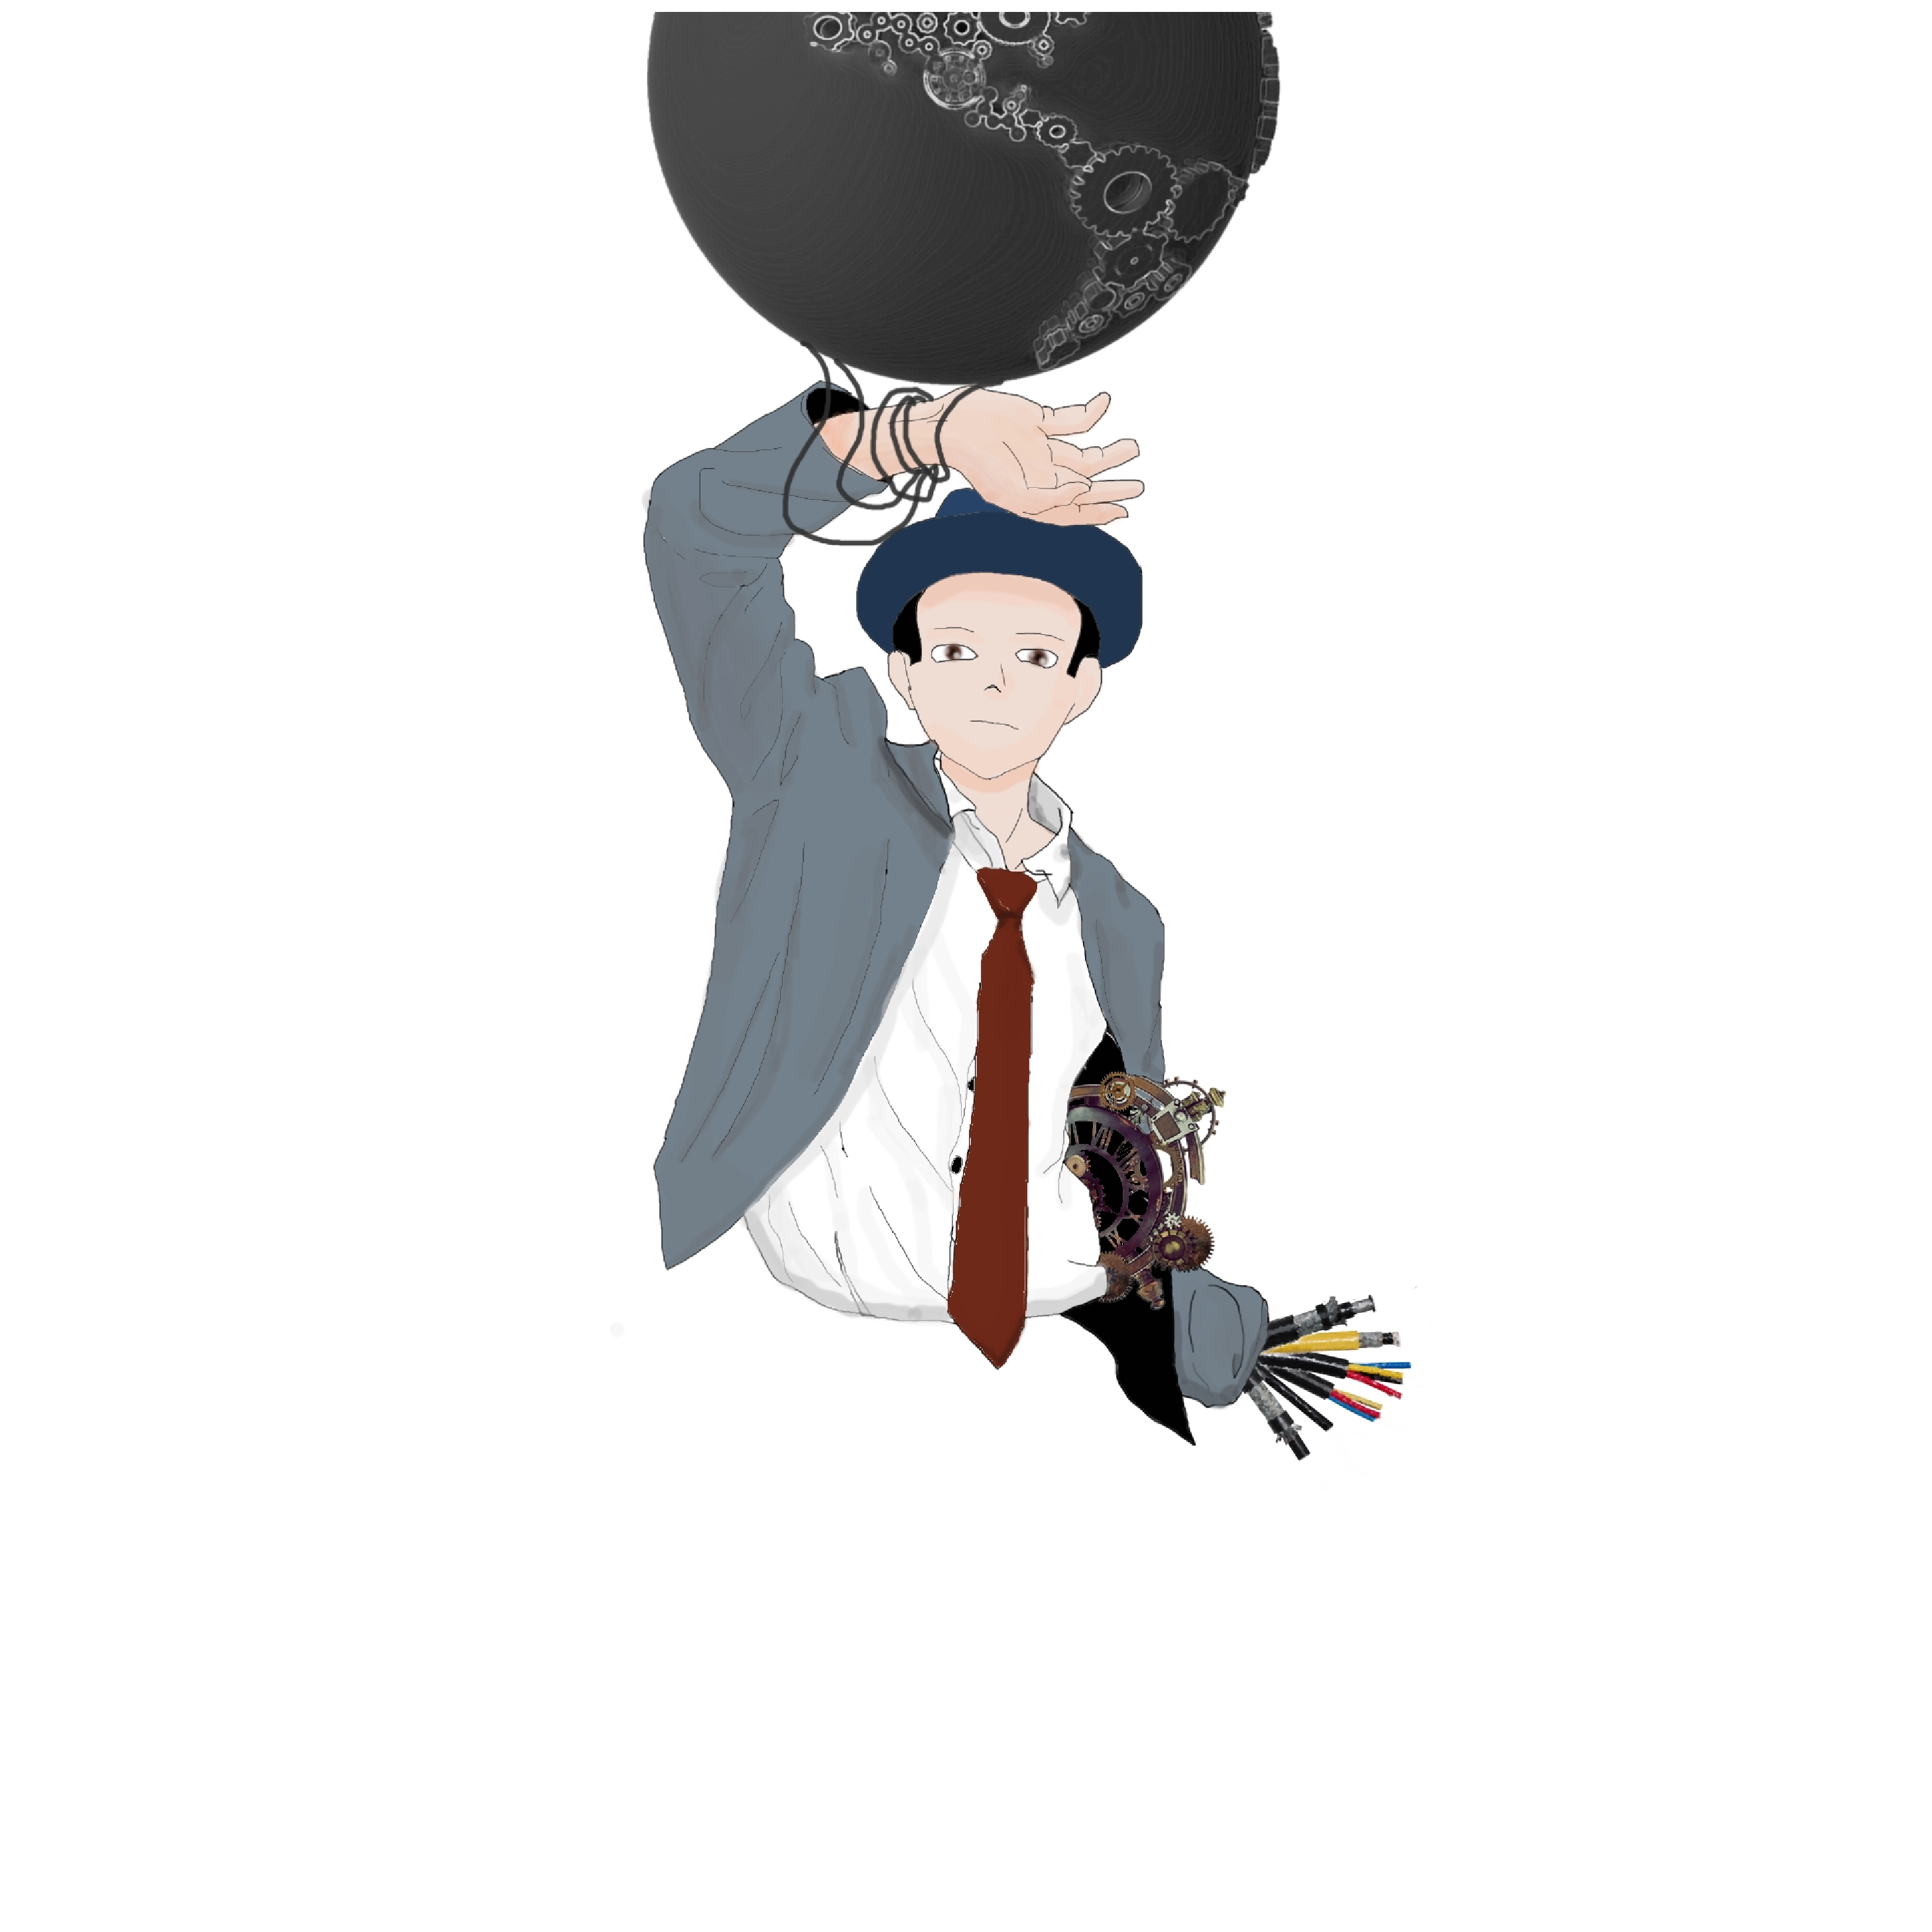
\includegraphics[width=0.85\columnwidth]{Imagenes/intro1.eps}
%\end{figure} 

\end{frame}


\subsection{Justificaci\'on}
\begin{frame}
\frametitle{Justificaci\'on}

\begin{table}
\scalebox{0.75}{
\begin{tabular}{|l||c|c|c|}
\hline

\textbf{A\~no} & \textbf{2010} & \textbf{2012} & \textbf{2014} \\
\hline\hline

\textbf{Poblaci\'on Total} & $113.4$ M & $117.4$ M & $118.3$ M \\
\hline

\textbf{Poblaci\'on con Discapacidad} & $5.6$ M & $7.7$ M & $7.1$ M \\
\hline

\textbf{Porcentaje de Discapacidad} & $5.0\%$ & $6.6\%$ & $6.0\%$ \\
\hline

\end{tabular}
}
\caption{Poblaci\'on con discapacidad en M\'exico, seg\'un distintas fuentes
 (Censo de Poblaci\'on y Vivienda de 2010, Encuesta Nacional de Ingresos y
 Gasto de los Hogares de 2012, Encuesta Nacional de la Din\'amica 
 Demogr\'afica 2014)\cite{Milosavljevic2014,INEGI2014}}
\label{PoblacionDis}
\end{table}

\vspace{-0.5cm}
\begin{block}{Mover o usar sus brazos o manos -- $33.0\%$}
\begin{columns}[T]
\begin{column}{.5\textwidth}
\begin{itemize}
\item {Enfermedad: $47.8\%$}
\item {Edad Avanzada: $29.2\%$}
\item {Accidente: $14.1\%$}
\end{itemize}
\end{column}

\begin{column}{.5\textwidth}
\begin{itemize}
\item {Nacimiento: $6.1\%$}
\item {Violencia: $0.5\%$}
\item {Otra causa: $2.3\%$}
\end{itemize}
\end{column}
\end{columns}
\end{block}

\end{frame}

\subsection{Planteamiento del problema}
\begin{frame}
\frametitle{Planteamiento del problema}

La poblaci\'on de Personas con Movilidad Reducida(PRM) va en aumento en 
 M\'exico  y con el uso de la computadora como algo imprescindible en la 
 actualidad, la discapacidad de estas personas puede representar un 
 obst\'aculo en su desarrollo laboral.

\end{frame}

\subsection{Hip\'otesis}
\begin{frame}
\frametitle{Hip\'otesis}

El ser humano es un ser de costumbres, por lo que hay tareas repetitivas
 que son automatizables, por tal, el uso del software a desarrollar
 permitir\'a al usuario de la PC agilizar este tipo de tareas, ayudando con 
 un manejo m\'as \'agil del equipo.

\end{frame}

\subsection{Propuesta de trabajo}
\begin{frame}
\frametitle{Propuesta de trabajo}

\footnotesize
\begin{itemize}
\item{Interacci\'on con todos los programas de un usuario}
\item{Facilidad de uso}
\item{Automatizar las acciones de un usuario}
\end{itemize}

\begin{figure}[h]
\centering
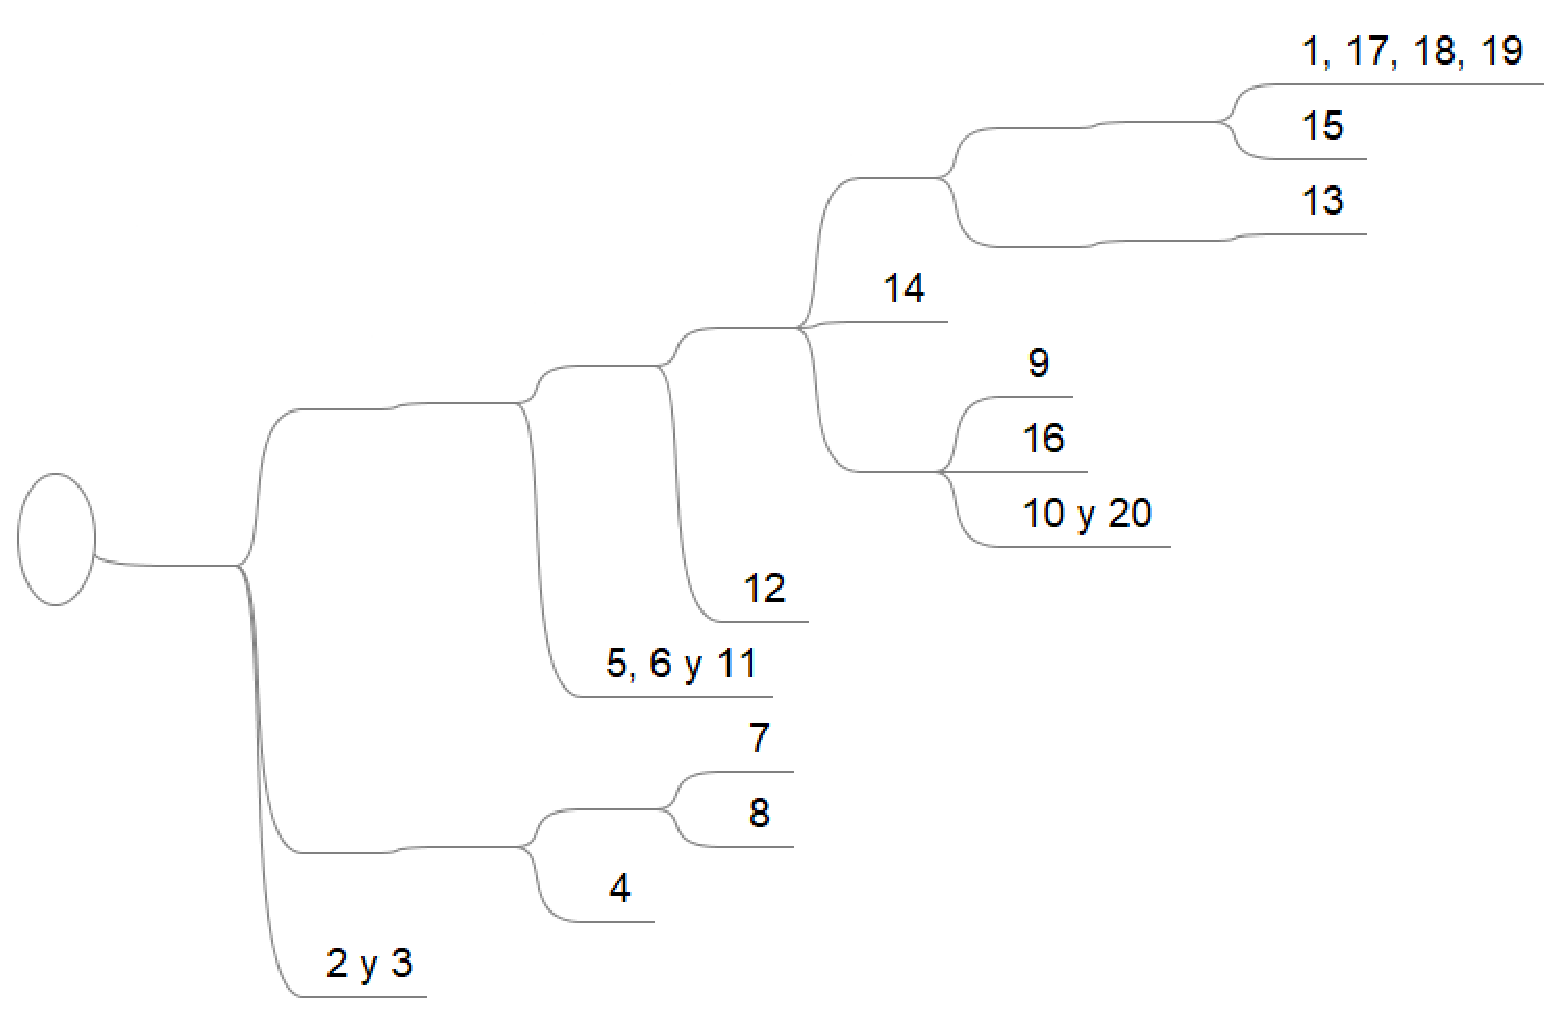
\includegraphics[width=0.6\columnwidth]{Imagenes/Arbol.eps}
\caption{\footnotesize Ejemplo del \'arbol ideal generado al pasar 20 d\'ias
 de uso en una PC.}
\label{fig:arbol}
\end{figure}

\end{frame}


\subsection{Objetivos} 
\begin{frame}
\frametitle{Objetivo general} 

Dise\~nar y desarrollar un software que defina a partir de un periodo de
 tiempo determinado el conjunto de acciones con mayor incidencia de uso por 
 un usuario realizadas en una computadora por un usuario, para su uso 
 posterior.

\begin{block}{Objetivos espec\'ificos} 			
\begin{itemize}
  \item Desarrollar un sistema para la captura de acciones, tanto del rat\'on
  como del teclado.
  \item Crear e implementar un \'arbol para resolver el problema.
  \item Obtener una muestra de las acciones realizadas con el teclado y el 
  rat\'on por un usuario en una computadora.
  \item Dise\~nar y desarrollar el algoritmo para la determinaci\'on de
  tareas repetitivas.
\end{itemize}
\end{block}
	
\end{frame}
